\documentclass[sigconf]{acmart}
\usepackage{booktabs}
\usepackage{amsmath}
\usepackage{tabularx}
\usepackage{needspace}
\usepackage{graphicx}
\usepackage{balance}
% The bundled legacy ACM class triggers an obsolete microtype footnote patch.
% Disabling only that patch avoids a harmless compiler warning.
\microtypesetup{nopatch=footnote}
\graphicspath{{}{sections/}{figures/}{../figures/}{assignments/assignment_1/figures/}}
\setlength{\emergencystretch}{1em}
\setcopyright{none}
\settopmatter{printacmref=false,printccs=false,printfolios=true}
\acmDOI{}
\acmISBN{}
\acmPrice{}
\acmConference[]{}{}{}
\acmYear{2026}
\copyrightyear{2026}
\renewcommand{\footnotetextcopyrightpermission}[1]{}
\fancyhead{}
\fancyfoot[C]{\thepage}

% Research question agreed with the team; the fitness criterion is the
% best individual, not the population-average aggregate score.
\newcommand{\researchquestion}{Can lexicase selection retain greater structural diversity over evolution and closer final target coverage than tournament selection at different tournament sizes, without worsening the best individual's aggregate fitness?}

\title{Compromise or Specialists: Who Gets to Be a Parent?\texorpdfstring{\\}{ }Lexicase Selection in Robot Morphology Evolution}
\author{Group 44}
\affiliation{\institution{Vrije Universiteit Amsterdam}\country{The Netherlands}}
\renewcommand{\shortauthors}{Group 44}

\begin{document}
\hypersetup{pageanchor=false,
  pdftitle={Compromise or Specialists: Who Gets to Be a Parent? Lexicase Selection in Robot Morphology Evolution},
  pdfauthor={Group 44}}
\IfFileExists{cover.tex}{\onecolumn
\thispagestyle{empty}
\begin{center}
\vspace*{1.0cm}
{\Large Vrije Universiteit Amsterdam\par}
\vspace{0.5cm}
{\large Evolutionary Computing\par}
\vspace{1.5cm}
{\LARGE\bfseries Compromise or Specialists:\par
Who Gets to Be a Parent?\par}
\vspace{0.4cm}
{\Large\bfseries Lexicase Selection in Robot Morphology Evolution\par}
\vspace{1.1cm}
{\large Standard Assignment 1: Evolving a Robot Body\par}
\vspace{0.6cm}
{\Large Group 44\par}
\vspace{0.9cm}
\begin{tabular}{ll}
\toprule
Team member & Student ID \\
\midrule
{[Name 1]} & {[Student ID 1]} \\
{[Name 2]} & {[Student ID 2]} \\
{[Name 3]} & {[Student ID 3]} \\
{[Name 4]} & {[Student ID 4]} \\
\bottomrule
\end{tabular}
\vfill
% TODO before submitting: fill in the names and student IDs above, and set
% this date to the submission date.
16 September 2026\par
\vspace*{0.6cm}
\end{center}
\clearpage
\twocolumn
\setcounter{page}{1}
}{}
\hypersetup{pageanchor=true,
  pdftitle={Compromise or Specialists: Who Gets to Be a Parent? Lexicase Selection in Robot Morphology Evolution},
  pdfauthor={Group 44}}

\begin{abstract}
We compare exact lexicase selection with binary tournament selection and a tournament calibrated to match lexicase's distinct-parent count, in the evolution of robot morphologies toward five targets. Across ten paired seeds per condition and 10,100 evaluations per run, lexicase maintained greater within-population morphological diversity and achieved lower final target-best distances than both tournament conditions. All evolutionary conditions outperformed equal-budget random search on best-individual fitness. Lexicase's best-individual aggregate fitness did not differ significantly from binary tournament selection but was significantly worse than that of the calibrated tournament. Approximately matching the number of distinct parents did not reproduce lexicase's diversity or coverage.
\end{abstract}
\keywords{lexicase selection, exploration--exploitation, morphological diversity, target coverage, robot evolution}
\maketitle
\pagestyle{plain}
\raggedbottom

% ===== INTRODUCTION =====
\section{Introduction}
We want a population of structurally different robot bodies that together resemble five targets, while maintaining the best single body's aggregate fitness. This is an exploration--exploitation problem: keep useful alternatives without losing progress on the objective \cite{crepinsek2013}. We call structural variation within a population \textbf{morphological diversity}, the body closest to a given single target its \textbf{target specialist}, and the body with the best aggregate score, low average distance with a penalty for uneven distances, the \textbf{compromise body}.

Both properties are worth seeking in their own right. A set of distinct good solutions can be an end in itself rather than a means to one best solution, as in quality-diversity search \cite{pugh2016}; in robotics, such a collection of solutions that are both diverse and high-performing is what allows a damaged robot to rapidly find an alternative high-performing behaviour \cite{cully2015}. Variety is usually obtained by weakening selection, which costs fitness, so we ask whether lexicase can retain it without that cost.

Tournament selection favours bodies with better aggregate scores; larger tournaments increase this pressure \cite{eiben2015}. Lexicase considers targets in a fresh random order for each parent \cite{spector2012,helmuth2015}. A uniquely best body on one target is selected whenever that target comes first, giving target-best bodies reproductive opportunities beyond aggregate ranking. Lexicase is known to widen diversity in genetic programming, but that evidence comes from evolving programs rather than bodies \cite{helmuth2016diversity}, so it motivates this comparison without settling it.

\textbf{Research question.} \emph{\researchquestion} Only parent selection changes among the three EA conditions.

Relative to binary tournament, we expect greater diversity within the population over the run (\textbf{H1}) and lower final target-specialist distances (\textbf{H2}), but similar or worse compromise-body fitness (\textbf{H3}). A tournament calibrated by distinct-parent counts should not reproduce lexicase's diversity and coverage (\textbf{H4}). The \textbf{baseline check} is that each EA outperforms equal-budget random search.

% ===== METHODS =====
% Keep the methods opening with the fitness definition.
\Needspace{11\baselineskip}
\section{Methods}
\subsection{Representation and objective}
ARIEL tree genomes encode a core, typed and rotated modules, and attachment faces, permitting direct subtree variation \cite{ariel2026}. Candidates have at most 21 nodes including the core. We use the five
course-provided target bodies, containing 7, 11, 15, 19 and 25 nodes;
their exact tree definitions are available in the versioned repository
\cite{assignment2026,group44}. For weighted tree edit distances $d_j(x)$, the minimised score is
\begin{equation}
F(x)=\bar d(x)+\sqrt{\tfrac{1}{5}\sum_{j=1}^{5}(d_j(x)-\bar d(x))^2},
\quad \bar d(x)=\tfrac{1}{5}\sum_{j=1}^{5}d_j(x).
\label{eq:fitness}
\end{equation}
The standard deviation is calculated across the five target distances for one body, with denominator 5, not across individuals. In the course metric \cite{assignment2026,zhang1989}, insertion, deletion, or type change costs 1; rotation-only change costs 0.5; identical labels cost 0. Faces order children but incur no separate cost. Distances are not normalised by target size. The 25-node target exceeds the candidate limit, so coverage is compared within targets, not across target sizes.

\subsection{Parent selection}
\textbf{Lexicase} starts with the whole population and shuffles the five targets for each parent. It keeps only bodies with the smallest distance to the first target, then repeats on the remaining candidates with successive targets. Selection stops at one body or, after all targets, chooses uniformly among ties \cite{spector2012,helmuth2015}. Aggregate fitness still determines elitism and the reported best body.

\textbf{Tournament} samples $k$ distinct individuals uniformly without replacement and returns the lowest-scoring body; random draw order breaks ties \cite{eiben2015}. Each parent pick is independent, so individuals can be selected repeatedly. Binary tournament ($k=2$) is the main comparator; the calibrated $k=40$ tournament is the control (Section~\ref{sec:baseline}). Changing $k$ changes pressure on aggregate fitness, whereas lexicase changes which target determines eligibility.

% Keep the subsection heading with a useful amount of its opening text.
\Needspace{6\baselineskip}
\subsection{Shared EA and parameter choices}
Encoding, targets, fitness, initialisation, variation, survivors and budget remain fixed across EAs (Table~\ref{tab:settings}); only parent selection varies.

Initial sizes are requested uniformly from 1--20 non-core modules; growth stops if no attachment remains. Each generation selects and copies parent pairs, exchanges random non-core subtrees with probability 0.7, and then gives each child one mutation attempt. One of the four mutation operators is sampled uniformly at random ($p=0.25$ each). Node replacement changes type and rotation, pruning incompatible descendants;
shrink replaces a subtree with a leaf; hoist promotes a descendant; and subtree replacement grafts a random branch requested to contain 1--3 non-core modules. A mutation attempt may leave the body unchanged.

Children exceeding 21 nodes are discarded before evaluation. Reproduction continues until 100 children are retained. All retained children are evaluated; the best parent then replaces the worst child. This generational scheme avoids ranking all survivors by aggregate fitness, which could remove lexicase's specialists; one elite preserves the best score.

\begin{table}[t]
\caption{Settings fixed across the three EA conditions.}
\label{tab:settings}
\centering
\begin{tabularx}{\columnwidth}{@{}lX@{}}
\toprule
Setting & Value \\
\midrule
Population / offspring & 100 / 100 \\
Generations & 100 after initialisation \\
Final seeds & 0--9, paired across EA conditions \\
Size limit & 20 modules plus core \\
Crossover / mutation & 0.7 per pair / one attempt per child \\
Survivors & 99 children and one parent elite \\
Evaluation budget & 10,100 per run, including initialisation \\
\bottomrule
\end{tabularx}
\end{table}

Population size and generations follow the assignment's suggested scale \cite{assignment2026}. Each of the four mutation operators is equally likely, so no operator weighting had to be tuned; tuning one could have favoured a condition and confounded the comparison. Crossover probability 0.7 permits recombined and non-recombined offspring.

\subsection{Baseline and calibrated control}
\label{sec:baseline}

First, three lexicase calibration runs
(seeds 100--102, 50 generations) provide populations on which lexicase
and tournaments with
$k\in\{2,5,10,15,20,25,30,40,50\}$ each make 100 parent selections.
Across the resulting 150 generation-level observations, lexicase
selected a mean of 7.69 distinct parents per 100 selections. The nearest settings were $k=40$ (8.52) and $k=50$ (6.83), almost
equidistant; we chose $k=40$, which selects less
narrowly and should therefore retain more diversity, making it the harder
test for H4. Using separate calibration seeds
prevents the final experimental outcomes from influencing the choice of
control. The complete calibration results are available in the
versioned repository \cite{group44}.

We then compare lexicase, binary tournament, the calibrated $k=40$
tournament and random search across ten paired seeds, with binary
tournament as the primary comparator. The calibrated tournament tests
whether approximately matching lexicase's reproductive concentration is
enough to reproduce its diversity and its coverage, how close the final
population gets to each target. Final runs also record
distinct-parent counts to evaluate the match.

Random search draws 101 independent batches of 100 bodies using the same
initialisation, size limit and fitness, retaining only a best-so-far record.
Every condition uses $100+100\times100=10{,}100$ objective evaluations, each computing five target
distances.

\subsection{Measurements, analysis and scope}
Conditions are \textbf{paired by seed} ($s=0,\ldots,9$): for each seed, all conditions begin with the same initial population. Seeds, rather than generations, are the independent experimental replicates.

We report means, sample SDs and mean paired differences. Because the runs are paired, we apply two-sided Wilcoxon signed-rank tests to within-seed differences \cite{wilcoxon1945}, without assuming normality.
With ten pairs, we compute the tests exactly using SciPy \cite{virtanen2020}. Across 19 comparisons, we apply Holm correction within each family of related tests at $\alpha=0.05$ to account for multiple testing \cite{holm1979}. H4 uses the calibrated-control contrasts in diversity and coverage.

\textbf{Morphological diversity (H1).} After survivor selection we sample 20 bodies without replacement and record $D_g$, the mean weighted tree edit distance over all 190 pairs, far cheaper than all 4,950 pairs of the population. Larger $D_g$ indicates greater structural variation. We report trajectories, final diversity and final population-mean size, and summarise each run post hoc by $\overline D=100^{-1}\sum_{g=1}^{100}D_g$, which measures average retained diversity.

\textbf{Target specialists and coverage (H2).} For each target, coverage is the smallest distance reached by any member of the final population, and any body attaining it is a specialist for that target. These minima measure collective coverage.

\textbf{Best-individual fitness (H3 and baseline check).} $B_g$ is the lowest aggregate score in generation $g$. Elitism makes it the best score found so far; curves show its mean and sample SD across seeds. Random search likewise reports its best-so-far score.

\textbf{Concentration (H4).} We average each run's distinct-parent count over generations 1--100.

\begin{figure*}[t]
  \centering
  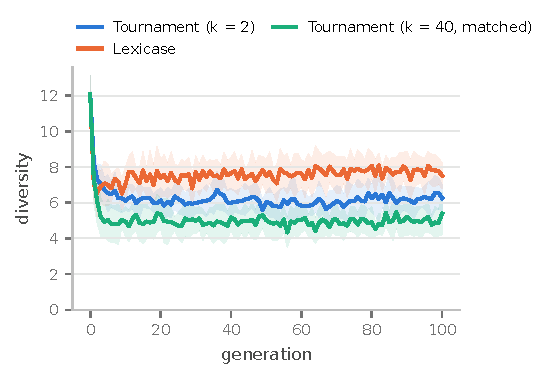
\includegraphics[width=0.48\textwidth]{diversity_curve.pdf}\hspace{2em}%
  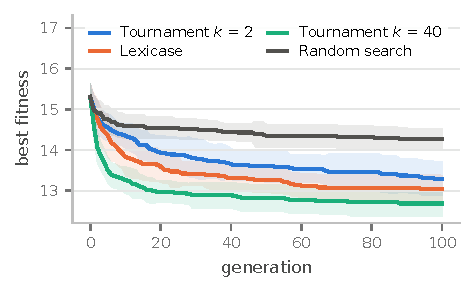
\includegraphics[width=0.48\textwidth]{fitness_curve.pdf}
  \caption{Left: within-population morphological diversity; higher means greater structural variation. Right: best-individual aggregate fitness $B_g$; lower is better. Lines show means across ten runs and bands show sample standard deviations. Generation 0 is the initial population.}
  \label{fig:trajectories}
\end{figure*}

% ===== RESULTS =====
\section{Results and Discussion}
All three measures use weighted tree-edit-distance units: lower is better for fitness and target distance, higher for diversity. Values are means over ten seeds, with the between-seed standard deviation in brackets: it measures spread, not quality. All $p$-values are Holm-adjusted.

\subsection{Calibration}
Calibration selected $k=40$: lexicase yielded 7.69 distinct parents per 100 picks, versus 8.52 for $k=40$, the closest tested setting. Final-run averages were 7.38 and 8.66, versus 56.90 for binary tournament. The control therefore approximates, but does not exactly match, lexicase's reproductive concentration.

\subsection{Morphological diversity}
Final diversity was 7.51 (0.72) for lexicase, 6.27 (0.74) for $k=2$ and 5.40 (1.19) for $k=40$. Lexicase was the more diverse in eight of ten matched seeds against binary tournament ($p=0.0098$) and in all ten against $k=40$ ($p=0.0039$), leading by 1.24 and 2.11 distance units on average. Averaged over the whole run the gap is wider and every seed favours lexicase (both $p=0.0039$): 7.55 (0.41) against 6.18 (0.48) for $k=2$ and 4.98 (0.57) for $k=40$. H1 therefore holds at the last generation and across the run (Figure~\ref{fig:trajectories}, left). Between the two tournaments, the larger $k$ was the less diverse (5.40 against 6.27, $p=0.0488$), the expected effect of stronger pressure on aggregate fitness. Random search was the most diverse condition of all, at 11.74 (0.96), and the worst on fitness, so diversity is not valuable in itself. What matters is diversity at comparable search quality, and there lexicase beat binary tournament with no significant difference in best fitness.



\subsection{Target coverage}

Lexicase achieved lower mean target-best distances on all five targets against both tournaments (all ten comparisons $p=0.0195$; Table~\ref{tab:coverage}), improving on binary tournament by 2.40 to 3.25 distance units. This supports H2 as \emph{collective} coverage: the population as a whole ends close to every target.

Random search is a sharper comparison than it first appears. It reached 3.35 on the 7-node target against binary tournament's 4.45, and tied at 11 nodes, so on the two smallest targets binary tournament gained nothing over sampling at random; lexicase beat random search on every target. Coverage comparisons with random search are descriptive.

Together with the diversity results, this supports H4: the $k=40$ control reproduces lexicase's number of distinct parents but neither its diversity nor its coverage. Which bodies reproduce therefore matters beyond how many.

\begin{table}[t]
\caption{Final target-specialist distance; values are mean (sample SD), lower is better. Random search reports the minimum over its final batch of 100 bodies, the same statistic over the same number of bodies as the evolved populations.}
\label{tab:coverage}
\centering
\scriptsize
\begin{tabular}{@{}lrrrr@{}}
\toprule
Target & Lexicase & $k=2$ & $k=40$ & Random \\
\midrule
7 nodes  & 2.05 (0.60) & 4.45 (0.86) & 5.15 (1.29) & 3.35 (0.24) \\
11 nodes & 3.90 (0.84) & 6.35 (0.34) & 7.15 (0.63) & 6.30 (0.89) \\
15 nodes & 5.65 (0.78) & 8.40 (0.70) & 8.95 (0.55) & 9.00 (0.75) \\
19 nodes & 8.85 (1.25) & 11.55 (0.83) & 10.90 (0.77) & 12.65 (0.53) \\
25 nodes & 10.80 (1.46) & 14.05 (0.86) & 12.65 (0.53) & 16.05 (0.96) \\
\bottomrule
\end{tabular}
\end{table}

\subsection{Best-individual fitness}

Final best fitness was 13.04 (0.34) for lexicase, 13.29 (0.42) for $k=2$, 12.69 (0.31) for $k=40$ and 14.27 (0.26) for random search. All three EAs improved on equal-budget random search (each $p=0.0059$), supporting the baseline check (Figure~\ref{fig:trajectories}, right). Against binary tournament lexicase was 0.25 units \emph{better} on average, though not significantly so ($p=0.1309$), so we found no fitness cost. Against the calibrated control lexicase was 0.36 units worse, and that gap is real ($p=0.0078$), though small: final scores run from 12.7 to 13.3, so 0.36 is under 3\% of them. H3 predicted similar or worse fitness, and both results fall inside it. The usual objection to diversity-preserving selection is that it trades away fitness; against the standard comparator we looked for that trade-off and did not find it. Better coverage need not improve individual fitness anyway: coverage takes a separate minimum per target, possibly from different bodies, whereas $F$ scores all five distances of one body.


% ===== CONCLUSIONS =====
\section{Conclusions}
Lexicase maintained greater morphological diversity and closer
collective target coverage than both tournaments. Best-individual
aggregate fitness was significantly worse than with $k=40$,
but did not differ significantly from binary tournament.
Approximately matching distinct-parent counts did not reproduce
lexicase's advantages, suggesting that which bodies reproduce
matters beyond how many. These findings are limited to ten seeds,
one target set, budget and survivor scheme, imperfect concentration
matching, and unmeasured specialist overlap. The nonsignificant
fitness difference does not establish equivalence.
Future work could vary target similarity to test when competing
specialists benefit coverage, and compare exact with
$\epsilon$-lexicase selection \cite{lacava2016epsilon}.
By retaining near-best candidates at each step,
$\epsilon$-lexicase could let more targets influence selection, changing
the balance between coverage and aggregate fitness.


\clearpage
\balance
\bibliographystyle{ACM-Reference-Format}
\bibliography{references}
\end{document}
